% !TEX TS-program = LuaLaTeX
\documentclass[11pt]{ltjsarticle}


%フォント(和文) japreset を使うことによって、一括に管理するようにしている。
\usepackage[hiragino-pron,jis2004,
deluxe%明朝体・ゴシック体各3ウェイトと,丸ゴシック体(mg)を利用可能にする
,bold%明朝体太字をゴシック体太字によって代替する.
]{luatexja-preset}
%\renewcommand{\kanjifamilydefault}{\gtdefault}% 既定をゴシック体に

\usepackage[height=8.8in,width=6.45in]{geometry}



%数式フォント
\usepackage{mathptmx}
\usepackage[scaled]{helvet}
\renewcommand{\ttdefault}{pcr}

\usepackage{mathtools} %extended amsmath
\usepackage{amssymb}
%\mathtoolsset{showonlyrefs=true,showmanualtags}%represent the number of equation when quote eqref
%\mathtoolsset{showonlyrefs,showmanualtags}
%\usepackage[warnings-off={mathtools-colon}]{unicode-math}


% not understanded
\countdef\cpart=1
\def\part#1{%
\newpage
\advance\cpart by 1
\section*{Part \the\cpart: #1}
\addcontentsline{toc}{section}{Part \the\cpart: #1}
%
}
\usepackage[nottoc]{tocbibind}

\usepackage{bm} %boldmath
\usepackage{mathdots}
\usepackage{ulem}


%????? これが効かないので一時的に外す。

\usepackage{graphicx} % include graphic
\usepackage{float}
\usepackage[svgnames]{xcolor}%(xcolor.pdf p38~39)

\usepackage{tensor}%for part 1 relativity

\usepackage{enumerate}
\usepackage{adjustbox}
\usepackage[
 unicode=true,
 colorlinks=true,
 bookmarks=true,
 bookmarksnumbered=true,
 pdftitle={notes},% タイトル
 pdfsubject={relativity},% サブタイトル
 pdfauthor={Shun Taniwaki},% 著者
 pdfkeywords={Weinberg-Cosmology}% キーワード
 citecolor=DarkGreen,
 linkcolor=FireBrick,
 %urlcolor=FireBrick,
 linktocpage=true,
]{hyperref}

%\usepackage{pxjahyper} ドライバ依存パッケージ
\usepackage[thref,amsmath,thmmarks]{ntheorem}

\theoremstyle{plain}
\theorembodyfont{\normalfont}
%\theoremsymbol{\text{\normalfont (Q.E.D.)}}
\theoremseparator{.}
\theoremstyle{break}

\usepackage{mdframed}
\newmdtheoremenv[ntheorem,backgroundcolor=black!10,linecolor=black!0]{principle}{原理}[section]
\newmdtheoremenv[ntheorem,backgroundcolor=black!10,linecolor=black!0]{assumption}{仮定}[section]
\newmdtheoremenv[ntheorem,backgroundcolor=black!10,linecolor=black!0]{definition}{定義}[section]
\newmdtheoremenv[ntheorem,backgroundcolor=black!10,linecolor=black!0]{formula}{公式}[section]
%\newmdtheoremenv[ntheorem,backgraoudcolor=black!0]{theorem}{定理}[subsection]
\newmdtheoremenv[ntheorem,backgroundcolor=black!10]{theorem}[definition]{事実}
\newmdtheoremenv[ntheorem,backgroundcolor=black!3,linecolor=black!0]{example}{(計算)例}[definition]
\newmdtheoremenv[ntheorem,backgroundcolor=black!0]{unclear}{Unclear points}[section]
%\newmdtheoremenv[mdframedoption]{envname}[numberedlike]{caption} [within]


\usepackage{tikz}
\usepackage[compat=1.1.0]{tikz-feynman} %前に配置すると、xcolorと喧嘩する。

\mathtoolsset{showonlyrefs,showmanualtags}

% def bold faces
\bmdefine{\bfa}{a}
\bmdefine{\bfb}{b}
\bmdefine{\bfc}{c}
\bmdefine{\bfd}{d}
\bmdefine{\bfe}{e}
\bmdefine{\bff}{f}
\bmdefine{\bfg}{g}
\bmdefine{\bfh}{h}
\bmdefine{\bfi}{i}
\bmdefine{\bfj}{j}
\bmdefine{\bfk}{k}
\bmdefine{\bfl}{l}
\bmdefine{\bfm}{m}
\bmdefine{\bfn}{n}
\bmdefine{\bfo}{o}
\bmdefine{\bfp}{p}
\bmdefine{\bfq}{q}
\bmdefine{\bfr}{r}
\bmdefine{\bfs}{s}
\bmdefine{\bft}{t}
\bmdefine{\bfu}{u}
\bmdefine{\bfv}{v}
\bmdefine{\bfw}{w}
\bmdefine{\bfx}{x}
\bmdefine{\bfy}{y}
\bmdefine{\bfz}{z}
\bmdefine{\bfA}{A}
\bmdefine{\bfB}{B}
\bmdefine{\bfC}{C}
\bmdefine{\bfD}{D}
\bmdefine{\bfE}{E}
\bmdefine{\bfF}{F}
\bmdefine{\bfG}{G}
\bmdefine{\bfH}{H}
\bmdefine{\bfI}{I}
\bmdefine{\bfJ}{J}
\bmdefine{\bfK}{K}
\bmdefine{\bfL}{L}
\bmdefine{\bfM}{M}
\bmdefine{\bfN}{N}
\bmdefine{\bfO}{O}
\bmdefine{\bfP}{P}
\bmdefine{\bfQ}{Q}
\bmdefine{\bfR}{R}
\bmdefine{\bfS}{S}
\bmdefine{\bfT}{T}
\bmdefine{\bfU}{U}
\bmdefine{\bfV}{V}
\bmdefine{\bfW}{W}
\bmdefine{\bfX}{X}
\bmdefine{\bfY}{Y}
\bmdefine{\bfZ}{Z}
\bmdefine{\bftheta}{\theta}
\bmdefine{\bfphi}{\varphi}
\bmdefine{\bfomega}{\omega}




%mathbf
\newcommand{\mbfa}{\mathbf{a}}
\newcommand{\mbfb}{\mathbf{b}}
\newcommand{\mbfc}{\mathbf{c}}
\newcommand{\mbfd}{\mathbf{d}}
\newcommand{\mbfe}{\mathbf{e}}
\newcommand{\mbff}{\mathbf{f}}
\newcommand{\mbfg}{\mathbf{g}}
\newcommand{\mbfh}{\mathbf{h}}
\newcommand{\mbfi}{\mathbf{i}}
\newcommand{\mbfj}{\mathbf{j}}
\newcommand{\mbfk}{\mathbf{k}}
\newcommand{\mbfl}{\mathbf{l}}
\newcommand{\mbfm}{\mathbf{m}}
\newcommand{\mbfn}{\mathbf{n}}
\newcommand{\mbfo}{\mathbf{o}}
\newcommand{\mbfp}{\mathbf{p}}
\newcommand{\mbfq}{\mathbf{q}}
\newcommand{\mbfr}{\mathbf{r}}
\newcommand{\mbfs}{\mathbf{s}}
\newcommand{\mbft}{\mathbf{t}}
\newcommand{\mbfu}{\mathbf{u}}
\newcommand{\mbfv}{\mathbf{v}}
\newcommand{\mbfw}{\mathbf{w}}
\newcommand{\mbfx}{\mathbf{x}}
\newcommand{\mbfy}{\mathbf{y}}
\newcommand{\mbfz}{\mathbf{z}}
\newcommand{\mbfA}{\mathbf{A}}
\newcommand{\mbfB}{\mathbf{B}}
\newcommand{\mbfC}{\mathbf{C}}
\newcommand{\mbfD}{\mathbf{D}}
\newcommand{\mbfE}{\mathbf{E}}
\newcommand{\mbfF}{\mathbf{F}}
\newcommand{\mbfG}{\mathbf{G}}
\newcommand{\mbfH}{\mathbf{H}}
\newcommand{\mbfI}{\mathbf{I}}
\newcommand{\mbfJ}{\mathbf{J}}
\newcommand{\mbfK}{\mathbf{K}}
\newcommand{\mbfL}{\mathbf{L}}
\newcommand{\mbfM}{\mathbf{M}}
\newcommand{\mbfN}{\mathbf{N}}
\newcommand{\mbfO}{\mathbf{O}}
\newcommand{\mbfP}{\mathbf{P}}
\newcommand{\mbfQ}{\mathbf{Q}}
\newcommand{\mbfR}{\mathbf{R}}
\newcommand{\mbfS}{\mathbf{S}}
\newcommand{\mbfT}{\mathbf{T}}
\newcommand{\mbfU}{\mathbf{U}}
\newcommand{\mbfV}{\mathbf{V}}
\newcommand{\mbfW}{\mathbf{W}}
\newcommand{\mbfX}{\mathbf{X}}
\newcommand{\mbfY}{\mathbf{Y}}
\newcommand{\mbfZ}{\mathbf{Z}}
%tilde
\newcommand{\tilg}{\tilde{g}}
\newcommand{\tilGamma}{\tilde{\Gamma}}
%****
\def\TODO#1{{\color{FireBrick} #1}}
%***
\newcommand{\Slash}[1]{{\ooalign{\hfil/\hfil\crcr$#1$}}}%スラッシュ引くよう

\def\ii{\mathrm{i}}
\def\Nequals#1{$\mathcal{N}{=}\,#1$}

%def tensors
\newcommand{\tensorR}[1]{\tensor{R}{ #1}}
\newcommand{\tensorGamma}[1]{\tensor{\Gamma}{ #1}}
\newcommand{\tensorG}[1]{\tensor{G}{ #1}}
\newcommand{\tensorg}[1]{\tensor{g}{ #1}}

%def math operators
\DeclareMathOperator{\arcsinh}{arcsinh}
\def\odi#1#2{\frac{d #1}{d #2}} %ordinary differential
\def\todi#1#2{\frac{d^{2} #1}{d #2^{2}}} %two ordinary differential
\newcommand{\pdi}[2]{\frac{\partial #1}{\partial #2}}%partial differential
\newcommand{\tpdi}[2]{\frac{\partial #1^{2}}{\partial #2^{2}}}%two partial differential
\def\vev#1{\Bigl(#1\Bigr)}% Vacume Expectation Value ?
\DeclareMathOperator{\sign}{sign}% sign
\def\diag{\mathop{\mathrm{diag}}\nolimits}% diagonalize
\def\tr{\mathop{\mathrm{tr}}\nolimits}% trace
\def\adj{\mathop{\mathrm{adj}}}% adjoint

%*********************************************************************

%def alert
\def\alert#1{\textbf{\textcolor{red}{\uwave{#1}}}}
%*********************************************************************

%\pagestyle{empty}
\begin{document}
\newpage
\section{クインテッセンス(Quintessence) (途中まで)}\label{sec1-12:Quintessence}

今まで、宇宙の膨張率を計算する際、非相対論的エネルギー、放射、そして、定数の真空エネルギーのみを考慮してきた。
真空エネルギーの密度は、場の量子論の理論に基づいて見積もった値に比べて、桁違いに小さい。
\footnote{これは、どういうことでしょうか。
自由なスカラー場の時の、$H= \int {(a^{\dagger}a +1/2)}$ で、$a^{\dagger}a = 0,1,2 \dots $で、この比に比べると大きいよね?、ということでしょうか。}
そして、現在の物質密度に比べて、2、3倍程度大きいくらいである。
この事実は、真空のエネルギーが実は定数ではないのではないか、という推測(憶測)を呼ぶこととなった。
そして、現時点の真空エネルギーが小さいのは宇宙が”古い”からだ、というのである。
このような、時間変動する真空エネルギーはしばしば、クインテッセンス(Quintessence)と呼ばれている。
\begin{definition}
クインテッセンス(Quintessence)とは、時間変動する真空エネルギーのことを言う。
\end{definition}

では、変動する真空エネルギーを導入しよう。
自然な方法は、スカラー場の存在を仮定することである。
真空のエネルギーはそれらのスカラー場の値に依存し、
スカラー場自身の期待値も時間とともに変化する。\footnote{説明しろ、と言われると詰まるので、説明できるようにしておく。}
この種のスカラー場は、現代の弱い相互作用(SU(2)ゲージ理論)と電磁相互作用(U(1)ゲージ理論)の理論で重要な役割を果たし、4章や、10章で議論するインフレーションにも導入されている。

簡単のため、一変数の実スカラー場$\varphi(\mbfx,t)$を考える。
$\varphi$をクインテッセンスの場だと思うということ。
この場は、素粒子のスケールでは変化が小さい。
その結果、これらの場の作用が、時空に関する微分(derivative)で最小となる。
ラグランジアン(Lagrangian)を
\begin{align}
  L = - \frac{1}{2} g^{\lambda \kappa} \frac{\partial \varphi}{\partial x^{\lambda}} \frac{\partial \varphi}{\partial x^{\kappa}}-V(\varphi)
\end{align}%
とすれば、作用(action)は、
\begin{align}
  I_{\varphi}=-\int d^{4} x \sqrt{-\operatorname{Detg}}\left[\frac{1}{2} g^{\lambda \kappa} \frac{\partial \varphi}{\partial x^{\lambda}} \frac{\partial \varphi}{\partial x^{\kappa}}+V(\varphi)\right]
\end{align}%
となる。
ポテンシャル$V(\phi)$の関数形は決めないでおく。
さて、僕らはRobertson–Walker 計量の場合に興味があるわけで、スカラー場は座標(position)によらずに、時間(time)のみに依るものとする。
さすれば、公式 (B.66、B.67) から、スカラー場のエネルギー密度および圧力は以下のようになる。
\begin{align}
  \rho_{\varphi}=&\frac{1}{2} \dot{\varphi}^{2}+V(\varphi) \label{eq:1.12.2}\\
   p_{\varphi}=&\frac{1}{2} \dot{\varphi}^{2}-V(\varphi) \label{eq:1.12.3}
\end{align}%
これより直ちに、$\rho_{\varphi}+p_{\varphi} = (1+w)\rho_{\varphi}  = \dot{\varphi}^2 \geq 0$が導かれる。
$\rho_{\varphi}\geq 0 $である限り、$1+w\geq0  \Leftrightarrow w \geq -1$となるので、1.6節で議論したファントムエネルギーの心配は、このモデルでは不要である。

エネルギー運動量保存則$T^{\mu\nu}{;\nu}$を考える。今はロバートソン・ウォーカーの場合を考えているから、$\dot{\rho} = -3H (p+\rho)$の式に上のスカラー場のエネルギー密度および圧力を代入すれば、
\begin{align}
  \ddot{\varphi}+3 H \dot{\varphi}+V^{\prime}(\varphi)=0 \label{eq:1.12.4}
\end{align}%
とかける。($H=H(t)=\dot{a}(t)/a(t)$)
この式は、上の作用の場の方程式も同じ結果を与える。\footnote{検算が必要。}
式変形して、
\begin{align}
  \ddot{\varphi}=-3 H \dot{\varphi}-  V^{\prime}(\varphi)
\end{align}%
とかけば、一次元座標$\varphi$をポテンシャル$V(\varphi)$と、速度$\dot{\varphi}$に比例する摩擦力$-3H\dot{\varphi}$のもとで運動する(単位質量粒子の)運動方程式と等価である。
これは、今、$\varphi$が時間にのみ依存するから、このような見方ができる。
場はポテンシャルが小さくなる方向に変化し、その変化は$V(\varphi)$が最小値、あるいは、最低でも局所最小値を持つ値に到達した時にとまる。グローバルミニマムか、ローカルミニマムで止まるということ。
残念ながら(?)、我々は、どうして$V(\varphi)$の値が停留するところで小さくなくてはならない理由をしらない。(どうゆうこと???)
(Unfortunately, we do not know any reason why the value of $V(\varphi)$ where it is stationary should be small.)
どう言うことでしょう、Wienberg 節だと思うことにして、次にすすむ。

Nevertheless, there are potentials that have some attractive properties once we adjust an additive constant in the potential to make them vanish at their stationary point.
和訳すると、
それにもかかわらず(nevertheless)、ポテンシャルに定数を加えるか差し引くかして調整してポテンシャルの停留点でにおけるポテンシャルの値を消しさえすれば(直訳したのでわかりずらくて、ポテンシャルの定数を加えるか引くかして調整して、最小値(または極小値)をゼロにしてやるようにさえすれば、ということで、話を続けると)、いくつかの有用な性質を持つポテンシャルを得ることができる、とのこと。
%僕は、文脈から察するに、ポテンシャルは0以上であるよ、と言っているように思えた。
%どんなポテンシャルを考えても良くて、そして、その最小値を定数の自由度を使ってゼロにしてあげる、すなわち、全体で見るとポテンシャルは0以上ということ。
%Nevertheless, there are potentials that have some attractive properties once we adjust an additive constant in the potential to make them vanish at their stationary point.
どういうことでしょう。
あまり重要ではなさそうだから、次に進む。
クインテッセンスモデルの元祖(original)で最も単純な(simplest)な例は、ポテンシャルが
\begin{align}
  V(\varphi)=M^{4+\alpha} \varphi^{-\alpha} \label{eq:1.12.5}
\end{align}%
で与えられる場合である。
ここで、$\alpha$は任意の正の定数で、$M$は$\hbar = c = 1$のもとでの定数、そして、これより$V$はエネルギー密度の次元を与える。
ポテンシャルがこの形をもつという特別な理由はないし、とりわけ、(他の全ての場の量子ゆらぎの効果を含む)$\phi = \infty$におけるポテンシャル$V$の値をノンゼロの値を与えるような、定数を加えたり差し引いたりする自由度をを除外する理由は知られていない。
そういった問題はあるにせよ、この特殊なクインテッセンスのモデルの帰結を見てみるのは有益だろう。
\footnote{ it may be illuminating to work out the consequences of this one specific model of quintessence.の訳。うまいと思う。}

どんなポテンシャルでも、十分に初期の宇宙では、$\rho_{\varphi} \ll \rho_{R}$でないといけない。
理由は3.2節までのお楽しみ。
少しだけここで説明すると、宇宙の元素合成の時期のエネルギー密度の増加が大きければ、現在観測されているヘリウムの量を超えてしまうから(らしい)。
また、これらの宇宙早期における、(ニュートリノ(neutrinos)のような、エネルギーが$k_{B} T$ 未満の粒子の)放射のエネルギー密度$\rho_{R}$は、非相対論的物質のエネルギー密度$\rho_{M}$より大きい。($\rho_{R}\gg \rho_{M}$)
したがって、放射優勢の宇宙を考えれば良いのであるから、$\rho \propto a^{-4} \rightarrow a(t)\propto \sqrt{t} (K=0 のフリードマン方程式より)$だから、$H(t)=1/(2t)$で、式\eqref{eq:1.12.4}は、
\begin{align}
  \ddot{\varphi}+\frac{3}{2 t} \dot{\varphi}-\alpha M^{4+\alpha} \varphi^{-\alpha-1}=0 \label{eq:1.12.6}
\end{align}%
この方程式は、解を$(定数)\times t^{\beta}$と仮定して代入して、定数部分と$\beta$を求めることができて、解:
\begin{align}
  \varphi=\left(\frac{\alpha(2+\alpha)^{2} M^{4+\alpha} t^{2}}{6+\alpha}\right)^{\frac{1}{2+\alpha}} \label{eq:1.12.7}
\end{align}%
を得る。$\dot{\varphi}^2 ,V(\varphi)\sim t^{-2\alpha/(2+\alpha)}$あるので、非常に早期における $\rho_{\varphi}$は$\rho_{R}$より小さかった($\rho_{\varphi}<\rho_{R}$)に違いない。
というのは、$\rho_{R} \propto t^{-2}$で、また、$\alpha $ は任意の正定値で$-2<-2\alpha/(\alpha+2)$だから。
ただ、この解は一意でない。
しかし、この解は(他のどのような解も$t$が増加するという意味で)アトラクターであることに注意せよ。(式\eqref{eq:1.12.6}の数値計算結果を図\ref{fig:calculation_of_eq:1.12.6}、図\ref{fig:calculation_of_eq:1.12.6_log}にのせた。)
\begin{figure}
  \centering
  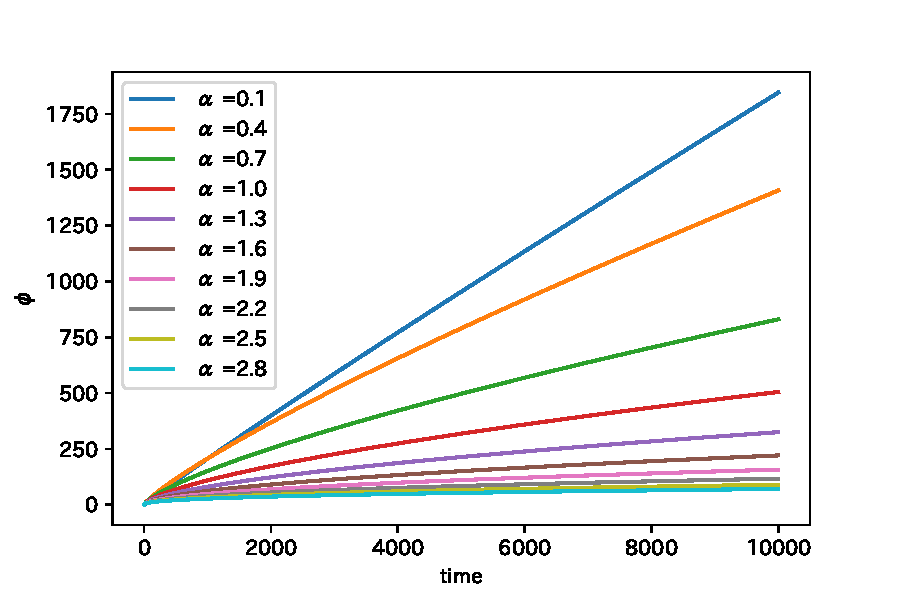
\includegraphics{figure/Attracter_cal.pdf}
  \caption{$\alpha$をいろいろ変えて式\eqref{eq:1.12.6}を数値計算。}
  \label{fig:calculation_of_eq:1.12.6}
  \centering
  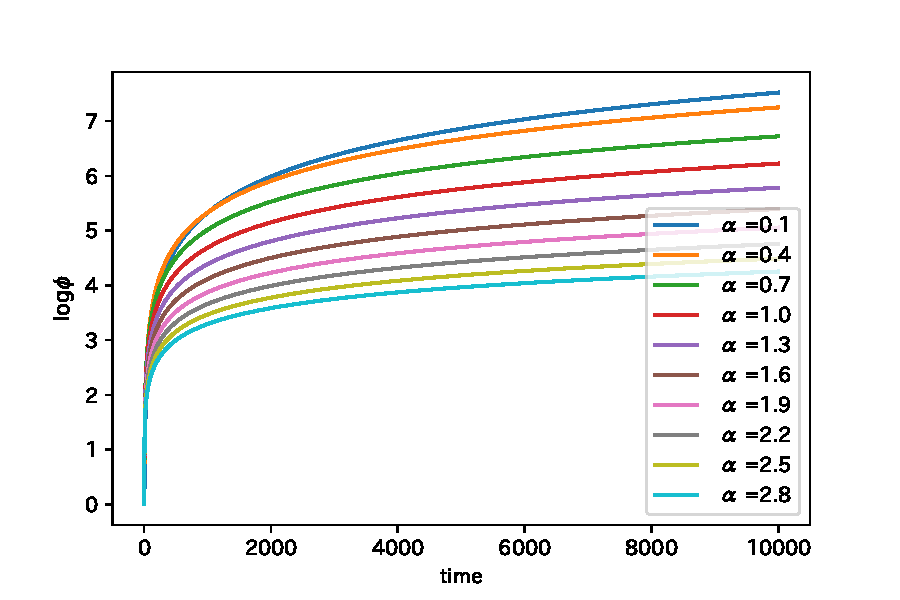
\includegraphics{figure/Attracter_cal_log.pdf}
  \caption{$\alpha$をいろいろ変えて式\eqref{eq:1.12.6}を数値計算の指数部分を見るために$\log$をとったもの。}
  \label{fig:calculation_of_eq:1.12.6_log}
\end{figure}%
これを理解するために、式\eqref{eq:1.12.7}で与えられる解に摂動$\delta \varphi$を与えてみよう($\varphi \to \varphi +\delta \varphi$)。
二階微分、一階微分の部分は線形だからそのままで、$\varphi^{-\alpha -1}\to(\varphi + \delta \varphi)^{-\alpha-1}\approx \varphi^{-\alpha -1} -(1+\alpha)\varphi^{-\alpha-2} \cdot \delta \varphi$
なので、これらより、$\varphi$は以下の式を満たす。
\begin{align}
  0=\delta \ddot{\varphi}+\frac{3}{2 t} \delta \dot{\varphi}+\alpha(1+\alpha) M^{4+\alpha} \varphi^{-\alpha-2} \delta \varphi=\delta \ddot{\varphi}+\frac{3}{2 t} \delta \dot{\varphi}+\frac{(6+\alpha)(1+\alpha)}{(2+\alpha)^{2} t^{2}} \delta \varphi
\end{align}%
そして、これは、$\delta\varphi = t^{\beta}$と解を仮定して代入すれば、
\begin{align}
  \delta \varphi \propto t^{\gamma}, \quad \gamma=-\frac{1}{4} \pm \sqrt{\frac{1}{16}-\frac{(6+\alpha)(1+\alpha)}{(2+\alpha)^{2}}}
\end{align}%
という形の二つの独立な解を得る。
$\alpha>0$なので、ルートの中身は負。少し計算するとわかる。
\begin{align}
  \frac{1}{16}-\frac{(6+\alpha)(1+\alpha)}{(2+\alpha)^{2}} = \frac{-15\alpha^2 - 92 \alpha -92}{16(\alpha+2)^2} < 0
\end{align}%
なので、平方根は$\alpha>0$で虚数を与えるから、$\delta \varphi$の解は、両方とも$t$が増加するとともに、$t^{-1/4}$のように減衰する。
この理由のため、$t\to0$において\footnote{文脈的に、$t$が増加すると、この解に近づくのだから、$t \to \infty$かと思ったがそうではないようだ。}、式\eqref{eq:1.12.7}のように振る舞う式\eqref{eq:1.12.6}の
特解は、トラッカー(tracker)解として知られている。
スカラー場の初期条件に対し、スカラー場が現在までにトラッカー解に近づくべしという条件(そのような初期条件は「アトラクションの内湾(basin of attraction)」と知られている)という物理的な理由は特にないのであるが、この要請によって、スカラー場の現在の進化が初期条件に依存しなくなるため、たった2つの自由パラメータ$M$と$\alpha$を持つクインテッセンスモデルが得られるという実用上の利便性がある。

放射のエネルギー密度が非相対論的物質のエネルギー密度を下回る時期が来ても、特に何も起こらない。
スカラー場のトラッカー解は、$t^{2/(2+\alpha)}$のように成長し、$\dot{\varphi}^2,V(\varphi)$は、$t^{-2\alpha(2+\alpha)}$のように減少し続ける。
しかし、$\rho_{M}$、$\rho_{R}$はそれぞれ$t^{-2}$、$t^{-8/3}$のようにより早く減少し続けるので、結果として、$\rho_{M}$と$\rho_{R}$が$\rho_{\varphi}$を下回るようになる($\rho_{R}<\rho_{M}\ll \rho_{\varphi}$)。
$\rho_{\varphi}=\rho_{M}$となる時刻での$\varphi$の値が、不明な定数$M$に依存しないのは興味深い。
これを以下では見ていく。
物質優勢での宇宙膨張の時、式(1.5.31)から、$\rho_M = 1/(6\pi G t^2)$と与えられるが、
式\eqref{eq:1.12.2}\footnote{英語版だと、1.1.2と誤植あり。}に、式\eqref{eq:1.12.5}および式\eqref{eq:1.12.7}を代入すれば、%\eqref{eq:1.5.31}$$
\begin{align}
  \rho_{\varphi} \approx M^{\frac{2(4+\alpha)}{2+\alpha}} t^{\frac{-2\alpha}{2+\alpha}}
\end{align}%
を与えるので、$\rho_{\varphi} = \rho_{M}$となる時刻$t_c$は、
\begin{align}
  t_c = \frac{1}{6\pi}\left(G^{-1} M^{\frac{-2(4+\alpha)}{2+\alpha}}\right)^{\frac{2+\alpha}{4}}\\
  t_c \approx M^{-\frac{4+\alpha}{2}} G^{-\frac{2+\alpha}{4}}
\end{align}%
で与えられ、これを式\eqref{eq:1.12.7}に代入すれば、以下の結果を得る。\footnote{僕の備忘録。計算で、$2+\alpha$の部分がうまく消える}
\begin{align}
  \varphi(t_c) \approx G^{-1/2}
\end{align}%

さて、少し状況を変える。$\rho_M$が$\rho_\varphi$を非常に下回れば($\rho_M\ll \rho_{\varphi}$)、式(1.5.37)の$H=\sqrt{\frac{8\pi G \rho_V}{3}}$より、式\eqref{eq:1.12.4}を考えれば、
\begin{align}
  \ddot{\varphi}+\sqrt{24 \pi G \rho_{\varphi}} \dot{\varphi}-\alpha M^{4+\alpha} \varphi^{-\alpha-1}=0
\end{align}%
$\rho_V \to \rho_\varphi$と置き換えた。$\rho_\varphi$は式\eqref{eq:1.12.2}で与えられる。
そして、この時代のトラッカー解は、複雑な時間依存性を持っている。
しかし、十分に時間が経過し、現在よりももっと後の時刻になれば(?)、再び単純な形をとることを見よう。
$\dot{\varphi}$に比例する減衰項は、$\varphi$の成長を妨げることから、最終的に$\dot{\varphi}$は$V(\varphi)$よりも小さくなり、また、$\ddot{\varphi}$に比例する慣性項は、減衰項やポテンシャル項に比べて、無視できるようになると推測できる(これは、4章と10章でのべるインフレーションの理論で重要な役割を果たす「スローロール(slow roll)」条件とよく似ている(らしい))。$\leftarrow$わからない。。。\dag

\end{document}


\section{Intergalactic absorption}\label{sec1-10:Intergalactic-absorption}
\section{Number counts}\label{sec:Number-counts}
\section{Horizons}\label{sec:Horizons}

\part{THE COSMIC MICROWAVE RADIATION BACKGROUND}
\section{Expectations and discovery of the microwave background}
\section{The equilibrium era}
\section{Recombination and last scattering}
\section{The dipole anisotorpy}
\section{The Sunyaev-Zel'dovich effect}
\section{Primary fluctuations in the microwave background: A first look}

\part{THE EARLY UNIVE
